

\tikzset{every picture/.style={line width=0.75pt}} %set default line width to 0.75pt        

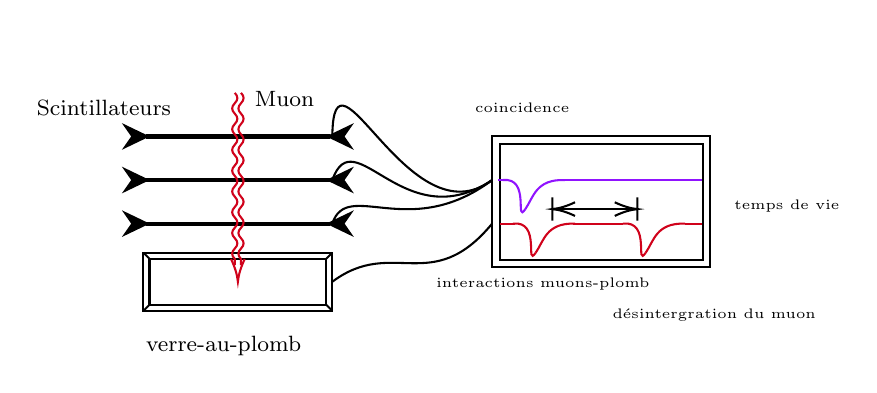
\begin{tikzpicture}[x=0.75pt,y=0.75pt,yscale=-1,xscale=1]
%uncomment if require: \path (0,300); %set diagram left start at 0, and has height of 300

%Straight Lines [id:da16127255456541323] 
\draw [color={rgb, 255:red, 0; green, 0; blue, 0 }  ,draw opacity=1 ][fill={rgb, 255:red, 245; green, 166; blue, 35 }  ,fill opacity=1 ][line width=1.5]    (176,49) -- (265,49) ;
\draw [shift={(263,49)}, rotate = 0] [fill={rgb, 255:red, 0; green, 0; blue, 0 }  ,fill opacity=1 ][line width=0.08]  [draw opacity=0] (13.4,-6.43) -- (0,0) -- (13.4,6.44) -- (8.9,0) -- cycle    ;
\draw [shift={(178,49)}, rotate = 180] [fill={rgb, 255:red, 0; green, 0; blue, 0 }  ,fill opacity=1 ][line width=0.08]  [draw opacity=0] (13.4,-6.43) -- (0,0) -- (13.4,6.44) -- (8.9,0) -- cycle    ;
%Straight Lines [id:da7982807003028938] 
\draw [color={rgb, 255:red, 0; green, 0; blue, 0 }  ,draw opacity=1 ][fill={rgb, 255:red, 245; green, 166; blue, 35 }  ,fill opacity=1 ][line width=1.5]    (176,70) -- (265,70) ;
\draw [shift={(263,70)}, rotate = 0] [fill={rgb, 255:red, 0; green, 0; blue, 0 }  ,fill opacity=1 ][line width=0.08]  [draw opacity=0] (13.4,-6.43) -- (0,0) -- (13.4,6.44) -- (8.9,0) -- cycle    ;
\draw [shift={(178,70)}, rotate = 180] [fill={rgb, 255:red, 0; green, 0; blue, 0 }  ,fill opacity=1 ][line width=0.08]  [draw opacity=0] (13.4,-6.43) -- (0,0) -- (13.4,6.44) -- (8.9,0) -- cycle    ;
%Straight Lines [id:da08370009723597649] 
\draw [color={rgb, 255:red, 0; green, 0; blue, 0 }  ,draw opacity=1 ][fill={rgb, 255:red, 245; green, 166; blue, 35 }  ,fill opacity=1 ][line width=1.5]    (176,91) -- (265,91) ;
\draw [shift={(263,91)}, rotate = 0] [fill={rgb, 255:red, 0; green, 0; blue, 0 }  ,fill opacity=1 ][line width=0.08]  [draw opacity=0] (13.4,-6.43) -- (0,0) -- (13.4,6.44) -- (8.9,0) -- cycle    ;
\draw [shift={(178,91)}, rotate = 180] [fill={rgb, 255:red, 0; green, 0; blue, 0 }  ,fill opacity=1 ][line width=0.08]  [draw opacity=0] (13.4,-6.43) -- (0,0) -- (13.4,6.44) -- (8.9,0) -- cycle    ;
%Shape: Bevel [id:dp6673775601267844] 
\draw   (175,105) -- (266,105) -- (266,133) -- (175,133) -- cycle ; \draw   (177.92,107.92) -- (263.08,107.92) -- (263.08,130.08) -- (177.92,130.08) -- cycle ; \draw   (175,105) -- (177.92,107.92) ; \draw   (266,105) -- (263.08,107.92) ; \draw   (266,133) -- (263.08,130.08) ; \draw   (175,133) -- (177.92,130.08) ;
%Straight Lines [id:da29762688824856964] 
\draw [color={rgb, 255:red, 208; green, 2; blue, 27 }  ,draw opacity=1 ]   (222,28) .. controls (223.67,29.67) and (223.67,31.33) .. (222,33) .. controls (220.33,34.67) and (220.33,36.33) .. (222,38) .. controls (223.67,39.67) and (223.67,41.33) .. (222,43) .. controls (220.33,44.67) and (220.33,46.33) .. (222,48) .. controls (223.67,49.67) and (223.67,51.33) .. (222,53) .. controls (220.33,54.67) and (220.33,56.33) .. (222,58) .. controls (223.67,59.67) and (223.67,61.33) .. (222,63) .. controls (220.33,64.67) and (220.33,66.33) .. (222,68) .. controls (223.67,69.67) and (223.67,71.33) .. (222,73) .. controls (220.33,74.67) and (220.33,76.33) .. (222,78) .. controls (223.67,79.67) and (223.67,81.33) .. (222,83) .. controls (220.33,84.67) and (220.33,86.33) .. (222,88) .. controls (223.67,89.67) and (223.67,91.33) .. (222,93) .. controls (220.33,94.67) and (220.33,96.33) .. (222,98) .. controls (223.67,99.67) and (223.67,101.33) .. (222,103) .. controls (220.33,104.67) and (220.33,106.33) .. (222,108) -- (222,111)(219,28) .. controls (220.67,29.67) and (220.67,31.33) .. (219,33) .. controls (217.33,34.67) and (217.33,36.33) .. (219,38) .. controls (220.67,39.67) and (220.67,41.33) .. (219,43) .. controls (217.33,44.67) and (217.33,46.33) .. (219,48) .. controls (220.67,49.67) and (220.67,51.33) .. (219,53) .. controls (217.33,54.67) and (217.33,56.33) .. (219,58) .. controls (220.67,59.67) and (220.67,61.33) .. (219,63) .. controls (217.33,64.67) and (217.33,66.33) .. (219,68) .. controls (220.67,69.67) and (220.67,71.33) .. (219,73) .. controls (217.33,74.67) and (217.33,76.33) .. (219,78) .. controls (220.67,79.67) and (220.67,81.33) .. (219,83) .. controls (217.33,84.67) and (217.33,86.33) .. (219,88) .. controls (220.67,89.67) and (220.67,91.33) .. (219,93) .. controls (217.33,94.67) and (217.33,96.33) .. (219,98) .. controls (220.67,99.67) and (220.67,101.33) .. (219,103) .. controls (217.33,104.67) and (217.33,106.33) .. (219,108) -- (219,111) ;
\draw [shift={(220.5,119)}, rotate = 270] [color={rgb, 255:red, 208; green, 2; blue, 27 }  ,draw opacity=1 ][line width=0.75]    (10.93,-3.29) .. controls (6.95,-1.4) and (3.31,-0.3) .. (0,0) .. controls (3.31,0.3) and (6.95,1.4) .. (10.93,3.29)   ;
%Curve Lines [id:da09987540810032502] 
\draw    (266,49) .. controls (266.44,-2.91) and (303,100) .. (343,70) ;
%Curve Lines [id:da8848703749954069] 
\draw    (266,91) .. controls (273.16,69.09) and (303,100) .. (343,70) ;
%Curve Lines [id:da6551396221292157] 
\draw    (266,70) .. controls (276.62,40) and (300.25,98.36) .. (343,70) ;
%Curve Lines [id:da5197903529881432] 
\draw    (266,119) .. controls (295.2,97.2) and (313.77,126.34) .. (343,91) ;
%Shape: Frame [id:dp11732449683870594] 
\draw   (343,49) -- (448,49) -- (448,112) -- (343,112) -- cycle(444.38,52.62) -- (346.62,52.62) -- (346.62,108.38) -- (444.38,108.38) -- cycle ;
%Curve Lines [id:da21062541779004906] 
\draw [color={rgb, 255:red, 208; green, 2; blue, 27 }  ,draw opacity=1 ]   (353,91) .. controls (366.77,89.34) and (358.63,112.63) .. (364,105) ;
%Curve Lines [id:da9677935870249211] 
\draw [color={rgb, 255:red, 144; green, 19; blue, 254 }  ,draw opacity=1 ]   (378,70) .. controls (364.06,69.49) and (362.91,78.34) .. (359,84) ;
%Curve Lines [id:da3394041776120852] 
\draw [color={rgb, 255:red, 208; green, 2; blue, 27 }  ,draw opacity=1 ]   (383,91) .. controls (369.06,90.49) and (367.91,99.34) .. (364,105) ;
%Curve Lines [id:da26392268148649634] 
\draw [color={rgb, 255:red, 208; green, 2; blue, 27 }  ,draw opacity=1 ]   (436,91) .. controls (422.06,90.49) and (420.91,99.34) .. (417,105) ;
%Curve Lines [id:da3170576792274794] 
\draw [color={rgb, 255:red, 144; green, 19; blue, 254 }  ,draw opacity=1 ]   (348,70) .. controls (361.77,68.34) and (353.63,91.63) .. (359,84) ;
%Curve Lines [id:da6469687920551798] 
\draw [color={rgb, 255:red, 208; green, 2; blue, 27 }  ,draw opacity=1 ]   (406,91) .. controls (419.77,89.34) and (411.63,112.63) .. (417,105) ;
%Straight Lines [id:da18630405985817278] 
\draw [color={rgb, 255:red, 144; green, 19; blue, 254 }  ,draw opacity=1 ]   (378,70) -- (444,70) ;
%Straight Lines [id:da8977881004274828] 
\draw [color={rgb, 255:red, 208; green, 2; blue, 27 }  ,draw opacity=1 ]   (382,91) -- (406,91) ;
%Straight Lines [id:da4750464176715349] 
\draw [color={rgb, 255:red, 208; green, 2; blue, 27 }  ,draw opacity=1 ]   (436,91) -- (444,91) ;
%Straight Lines [id:da15684561527929552] 
\draw [color={rgb, 255:red, 208; green, 2; blue, 27 }  ,draw opacity=1 ]   (347,91) -- (354,91) ;
%Straight Lines [id:da7885483833241824] 
\draw [color={rgb, 255:red, 144; green, 19; blue, 254 }  ,draw opacity=1 ]   (346,70) -- (350,70) ;
%Straight Lines [id:da39695529554469833] 
\draw    (372,84) -- (413,84) ;
\draw [shift={(413,84)}, rotate = 180] [color={rgb, 255:red, 0; green, 0; blue, 0 }  ][line width=0.75]    (0,5.59) -- (0,-5.59)(10.93,-3.29) .. controls (6.95,-1.4) and (3.31,-0.3) .. (0,0) .. controls (3.31,0.3) and (6.95,1.4) .. (10.93,3.29)   ;
\draw [shift={(372,84)}, rotate = 0] [color={rgb, 255:red, 0; green, 0; blue, 0 }  ][line width=0.75]    (0,5.59) -- (0,-5.59)(10.93,-3.29) .. controls (6.95,-1.4) and (3.31,-0.3) .. (0,0) .. controls (3.31,0.3) and (6.95,1.4) .. (10.93,3.29)   ;

% Text Node
\draw (169,35) node   [align=left] {\begin{minipage}[lt]{68pt}\setlength\topsep{0pt}
\footnotesize{Scintillateurs}
\end{minipage}};
% Text Node
\draw (274,31) node   [align=left] {\begin{minipage}[lt]{68pt}\setlength\topsep{0pt}
\footnotesize{Muon}
\end{minipage}};
% Text Node
\draw (228,150) node   [align=left] {\begin{minipage}[lt]{77.52pt}\setlength\topsep{0pt}
\footnotesize{verre-au-plomb}
\end{minipage}};
% Text Node
\draw (367.5,120) node   [align=left] {{\tiny interactions muons-plomb}};
% Text Node
\draw (450,135) node   [align=left] {{\tiny désintergration du muon}};
% Text Node
\draw (357.5,35) node   [align=left] {{\tiny coincidence}};
% Text Node
\draw (485,90) node   [align=left] {{\tiny temps de vie}\\};


\end{tikzpicture}
